% =====================================================================
%  V2V-Project -- Study Pack
%  Section S2 : Public Key Infrastructure / Certificate Authority
%  Source files studied: ca/ca.py , ca/issue_cert.py , ca/verify_cert.py
%  Standalone document -- compile with:  pdflatex 02-pki-certificate-authority.tex
% =====================================================================
\documentclass[11pt,a4paper]{article}

\usepackage[utf8]{inputenc}
\usepackage[T1]{fontenc}
\usepackage{lmodern}

\usepackage[a4paper,margin=2.4cm]{geometry}
\usepackage{enumitem}
\setlist{topsep=2pt,itemsep=2pt}

\usepackage{amsmath}
\usepackage{amssymb}
\usepackage{booktabs}
\usepackage{graphicx}
\usepackage{xcolor}
\usepackage{listings}
\usepackage{tikz}
\usetikzlibrary{arrows.meta,positioning,shapes.geometric,calc,fit,backgrounds}
\usepackage[colorlinks=true,linkcolor=blue,urlcolor=blue,citecolor=blue]{hyperref}

\definecolor{codebg}{rgb}{0.97,0.97,0.94}
\definecolor{codegreen}{rgb}{0.00,0.50,0.00}
\definecolor{codegray}{rgb}{0.50,0.50,0.50}
\definecolor{keyblue}{rgb}{0.00,0.20,0.70}
\definecolor{boxblue}{rgb}{0.88,0.93,1.00}
\definecolor{boxyellow}{rgb}{1.00,0.97,0.85}

\lstdefinestyle{py}{
  language=Python,
  backgroundcolor=\color{codebg},
  basicstyle=\ttfamily\footnotesize,
  keywordstyle=\color{keyblue}\bfseries,
  stringstyle=\color{codegreen},
  commentstyle=\color{codegray}\itshape,
  numberstyle=\tiny\color{codegray},
  numbers=left,
  numbersep=8pt,
  showstringspaces=false,
  breaklines=true,
  breakatwhitespace=false,
  frame=single,
  rulecolor=\color{codegray},
  tabsize=4,
  captionpos=b,
}
\lstdefinestyle{term}{
  backgroundcolor=\color{codebg},
  basicstyle=\ttfamily\footnotesize,
  breaklines=true,
  frame=single,
  rulecolor=\color{codegray},
  numbers=none,
  captionpos=b,
}

\title{\textbf{V2V-Project Study Pack}\\[4pt]
       \large Section S2 --- Public Key Infrastructure /\\ Certificate Authority}
\author{Information Security Project --- Beginner Study Notes}
\date{Source files: \texttt{ca/ca.py}, \texttt{ca/issue\_cert.py}, \texttt{ca/verify\_cert.py}}

\begin{document}
\maketitle
\tableofcontents
\newpage

% =====================================================================
\section{Title and ``What You'll Learn''}
% =====================================================================

\subsection*{Section Title}
\textbf{S2 --- The Public Key Infrastructure (PKI): how the project creates a
trusted ``passport office'' and issues digital passports to vehicles.}

\subsection*{Plain-English Summary (read this first)}
Before two cars can trust each other, each one needs a digital \emph{identity}
that cannot be faked. Section~S2 builds that identity system. A special program,
the \textbf{Certificate Authority (CA)}, acts like a passport office: it creates
its own master signing key and a self-signed master certificate, and then
\emph{signs} a small certificate for each vehicle. Any car can later check
another car's certificate by verifying the CA's signature on it --- if the CA
did not sign it, it is a fake. Three Python files do this work: \texttt{ca.py}
creates the CA, \texttt{issue\_cert.py} signs a certificate for one vehicle, and
\texttt{verify\_cert.py} checks a certificate.

\subsection*{Learning Outcomes}
After studying this section you will be able to:
\begin{itemize}
  \item Explain what \textbf{public-key (asymmetric) cryptography} is and why a
        key comes in a public/private pair.
  \item Explain \textbf{elliptic-curve cryptography} and the NIST \textbf{P-256}
        curve at a beginner level.
  \item Explain \textbf{SHA-256 hashing} and \textbf{ECDSA digital signatures}.
  \item Describe an \textbf{X.509 certificate}, its main fields, and the
        \textbf{BasicConstraints} and \textbf{KeyUsage} extensions.
  \item Explain \textbf{PEM, DER and Base64} encodings.
  \item Explain \textbf{PKI}, the \textbf{chain of trust}, a \textbf{trust
        anchor}, and a \textbf{self-signed root}.
  \item Walk through every function in \texttt{ca.py}, \texttt{issue\_cert.py}
        and \texttt{verify\_cert.py} and say what each line does.
  \item Run the three scripts, read their output, and explain how this stage
        defeats a man-in-the-middle attacker using a forged certificate.
\end{itemize}

% =====================================================================
\section{Where This Fits}
% =====================================================================

S2 is \textbf{Stage~1: Identity} of the three-stage pipeline. It comes first
because authentication (Stage~2) and secure messaging (Stage~3) are both built
\emph{on top of} the certificates created here. The handshake in S4 does not
re-invent identity --- it simply calls a verification routine that checks the
certificates this section produced.

\begin{center}
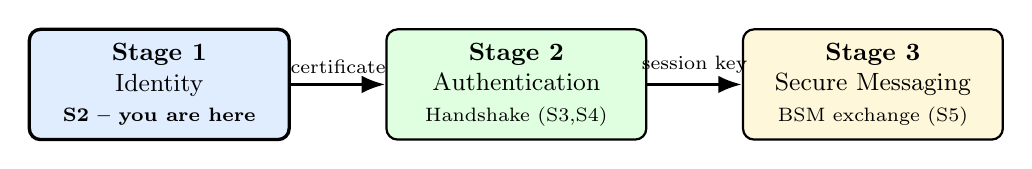
\begin{tikzpicture}[node distance=10mm and 12mm,every node/.style={font=\small},
    stage/.style={draw,rounded corners,minimum width=3.3cm,minimum height=1.4cm,
                  align=center,thick}]
  \node[stage,fill=boxblue,very thick]   (id)   {\textbf{Stage 1}\\Identity\\\scriptsize \textbf{S2 -- you are here}};
  \node[stage,fill=green!12,right=of id]   (auth) {\textbf{Stage 2}\\Authentication\\\scriptsize Handshake (S3,S4)};
  \node[stage,fill=boxyellow,right=of auth] (msg) {\textbf{Stage 3}\\Secure Messaging\\\scriptsize BSM exchange (S5)};
  \draw[-{Latex[length=3mm]},very thick] (id)   -- (auth)
       node[midway,above,font=\scriptsize]{certificate};
  \draw[-{Latex[length=3mm]},very thick] (auth) -- (msg)
       node[midway,above,font=\scriptsize]{session key};
\end{tikzpicture}
\end{center}

\noindent The \emph{certificate} produced here is the bridge into Stage~2: the
handshake hands a certificate to the other vehicle as proof of identity.

% =====================================================================
\section{The Theory You Must Study}
% =====================================================================

\subsection{Symmetric vs Asymmetric (Public-Key) Cryptography}
\textbf{Plain definition.} \emph{Symmetric} cryptography uses \emph{one} secret
key for both locking and unlocking --- both sides must already share it.
\emph{Asymmetric} (or \emph{public-key}) cryptography uses a \emph{pair} of
keys: a \textbf{private key} kept secret, and a \textbf{public key} given to
everyone. What one key does, only the other can undo.

\textbf{Real-life analogy.} Symmetric is one house key that both you and your
flatmate carry. Asymmetric is a mailbox: anyone can drop a letter through the
public slot, but only you have the private key to open the box and read it.

\textbf{Why it exists.} Symmetric keys have a chicken-and-egg problem: how do two
strangers agree on a shared secret over an untrusted channel \emph{without}
already having a secret? Public-key cryptography solves this --- you can publish
your public key to the whole world and it is still safe.

\textbf{How it works here.} Every key in S2 is a public/private \emph{pair}. The
CA has a pair; each vehicle has a pair. The private key is used to \emph{sign};
the public key is used to \emph{verify}. The certificate is simply a wrapper
that publishes a public key together with a name.

\textbf{Security property it provides.} Public-key cryptography underpins
\textbf{authentication} and \textbf{non-repudiation}.

\subsection{Elliptic-Curve Cryptography (ECC) and the P-256 Curve}
\textbf{Plain definition.} ECC is a family of public-key algorithms whose
security comes from the difficulty of a particular kind of arithmetic done on a
curved mathematical shape called an \emph{elliptic curve}.

\textbf{Real-life analogy.} Think of points hopping around a closed loop
according to a fixed rule. Going \emph{forwards} a known number of hops is easy;
working out \emph{how many hops} someone took just by seeing where they landed
is practically impossible. The private key is ``the number of hops''; the public
key is ``where you landed''.

\textbf{Why it exists.} An older algorithm, RSA, needs very large keys (2048+
bits) for strong security. ECC reaches the same strength with much smaller keys
(256 bits) --- so it is faster and the certificates and signatures are smaller,
which matters for cars sending messages many times a second.

\textbf{How it works here.} The project uses the curve named \texttt{SECP256R1},
also called \textbf{NIST P-256}. Both \texttt{ca.py} and \texttt{issue\_cert.py}
call \texttt{generate\_private\_key(SECP256R1())} to create keys on this curve.
P-256 gives a ``128-bit security level'' --- strong enough for decades --- and
it is the same curve used by TLS~1.3 (the security behind HTTPS).

\textbf{Security property it provides.} ECC is the engine under
\textbf{authentication} (via ECDSA signatures) and the key exchange in S3/S4.

\subsection{SHA-256 Hashing}
\textbf{Plain definition.} A \emph{hash function} takes any amount of data and
produces a short, fixed-size fingerprint of it. SHA-256 always produces 256 bits
(32 bytes). The same input always gives the same fingerprint; changing one bit
of input changes the fingerprint completely and unpredictably.

\textbf{Real-life analogy.} A paper shredder that always outputs the same-size
pile of confetti --- but a magic one, where identical documents always give an
identical pile, and you cannot rebuild the document from the confetti.

\textbf{Why it exists.} It is far faster to sign or compare a tiny 32-byte
fingerprint than a huge document, and the fingerprint reliably represents the
whole document.

\textbf{How it works here.} When the CA signs a certificate it does not sign the
raw certificate bytes directly --- it signs their SHA-256 hash. The code shows
this as \texttt{algorithm=hashes.SHA256()} passed to the \texttt{sign} call, and
\texttt{issue\_cert.py} also uses SHA-256 to compute a human-readable
\emph{fingerprint} of the finished certificate.

\textbf{Security property it provides.} Hashing supports \textbf{integrity}: any
change to the certificate changes its hash, so the signature no longer matches.

\subsection{Digital Signatures and ECDSA}
\textbf{Plain definition.} A digital signature is a short value, produced with a
\emph{private} key, that anyone holding the matching \emph{public} key can check.
ECDSA (Elliptic Curve Digital Signature Algorithm) is the elliptic-curve version.

\textbf{Real-life analogy.} A wax seal on a letter. Only the owner of the unique
seal-ring (private key) can press a genuine seal; anyone can look at the seal and
recognise it (public key) without owning the ring.

\textbf{Why it exists.} It answers two questions at once: ``who really wrote
this?'' (authentication) and ``has it been changed since?'' (integrity) --- and
because only the owner could have signed it, they cannot later deny it
(non-repudiation).

\textbf{How it works here.} \emph{Signing:} the CA computes the SHA-256 hash of
the certificate body and, using its private key and the P-256 curve, produces a
signature. \emph{Verifying:} a vehicle takes the certificate body, re-hashes it,
and uses the CA's \emph{public} key to confirm the signature matches. In
\texttt{verify\_cert.py} this is the line
\texttt{ca\_public\_key.verify(certificate.signature,
certificate.tbs\_certificate\_bytes, ec.ECDSA(...))}.

\textbf{Security property it provides.} \textbf{Authentication},
\textbf{integrity} and \textbf{non-repudiation}.

\subsection{X.509 Certificates}
\textbf{Plain definition.} An X.509 certificate is a standard-format digital
document that \emph{binds} a public key to an identity, and is \emph{signed} by
an issuer so others can trust the binding.

\textbf{Real-life analogy.} A passport. It contains your photo and name (the
identity), is printed in a worldwide standard format, and carries the issuing
government's tamper-proof features (the signature). A passport with no government
features is just a booklet --- worthless.

\textbf{Why it exists.} A bare public key is just a number --- it does not say
\emph{whose} key it is. The certificate attaches a name (``vehicle-a'') to the
key and has a trusted party vouch for that attachment.

\textbf{How it works here.} A certificate in this project contains:
\begin{itemize}
  \item \textbf{Subject} --- who the certificate is about (e.g.\ Common Name
        \texttt{vehicle-a}, Organisation \texttt{V2V-Security-Lab}).
  \item \textbf{Issuer} --- who signed it (the CA, \texttt{V2V-Root-CA}).
  \item \textbf{Public key} --- the subject's P-256 public key.
  \item \textbf{Serial number} --- a unique random number for this certificate.
  \item \textbf{Validity period} --- ``not valid before'' and ``not valid
        after'' dates.
  \item \textbf{Extensions} --- extra rules: BasicConstraints and KeyUsage.
  \item \textbf{Signature} --- the issuer's ECDSA signature over all of the above.
\end{itemize}

\textbf{Security property it provides.} The foundation of \textbf{authentication}.

\subsection{Certificate Extensions: BasicConstraints and KeyUsage}
\textbf{Plain definition.} Extensions are extra fields that state \emph{rules}
about how a certificate may be used. Each extension can be marked
\textbf{critical}, meaning a verifier that does not understand it must reject the
certificate.

\textbf{BasicConstraints} answers: ``Is this a Certificate Authority?''
\begin{itemize}
  \item For the CA: \texttt{ca=True} --- yes, it is allowed to sign \emph{other}
        certificates.
  \item For a vehicle: \texttt{ca=False} --- no, a vehicle may not sign
        certificates for anyone else.
\end{itemize}

\textbf{KeyUsage} answers: ``What is this key allowed to do?''
\begin{itemize}
  \item For the CA: \texttt{key\_cert\_sign=True} --- the only thing the CA key
        may do is sign certificates.
  \item For a vehicle: \texttt{digital\_signature=True} --- the vehicle key may
        sign data (used later in the handshake and BSM signing).
\end{itemize}

\textbf{Real-life analogy.} BasicConstraints is the difference between a
\emph{passport office} (may issue passports) and a \emph{citizen} (may not).
KeyUsage is like a driving licence that says ``car only, not motorbike''.

\textbf{Why it exists.} Without these limits, a stolen vehicle certificate could
be abused to issue fake certificates for a whole fleet. The constraints box each
key into exactly one job.

\textbf{Security property it provides.} It strengthens \textbf{authentication}
by preventing privilege escalation (a vehicle pretending to be a CA).

\subsection{Encodings: Base64, DER and PEM}
\textbf{Plain definition.}
\begin{itemize}
  \item \textbf{DER} (Distinguished Encoding Rules) is the compact \emph{binary}
        form of a certificate or key --- raw bytes.
  \item \textbf{Base64} is a way of writing binary bytes using only 64 ordinary
        printable letters/digits, so binary survives being copied as text.
  \item \textbf{PEM} (Privacy-Enhanced Mail) wraps Base64 text between header and
        footer lines such as \texttt{-----BEGIN CERTIFICATE-----} and
        \texttt{-----END CERTIFICATE-----}.
\end{itemize}

\textbf{Real-life analogy.} DER is a delicate object; Base64 is bubble-wrapping
it so it travels safely; PEM is the labelled cardboard box with ``BEGIN'' and
``END'' written on the flaps.

\textbf{Why it exists.} Binary bytes can be corrupted by e-mail, text editors or
copy-paste. PEM text survives all of that, and the BEGIN/END labels make it
obvious what is inside.

\textbf{How it works here.} Every file the CA writes ends in \texttt{.pem}. The
code calls \texttt{certificate.public\_bytes(serialization.Encoding.PEM)} and
\texttt{private\_key.private\_bytes(encoding=serialization.Encoding.PEM, ...)}.
When loading, it calls \texttt{x509.load\_pem\_x509\_certificate(...)}.

\textbf{Security property it provides.} None directly --- encoding is about
\emph{format}, not secrecy. (A PEM file is still readable; secrecy of a private
key comes from keeping the file itself protected.)

\subsection{PKI, the Chain of Trust, and the Self-Signed Root}
\textbf{Plain definition.} A \textbf{Public Key Infrastructure (PKI)} is the
whole system of authorities, certificates and rules that lets strangers trust
each other's public keys. A \textbf{chain of trust} is the line of signatures
from a certificate you are checking back to one you already trust. A
\textbf{trust anchor} (or \textbf{root}) is that already-trusted starting point.

\textbf{Real-life analogy.} You trust a stranger's passport because you trust the
\emph{country} that issued it --- you do not need to personally know the
stranger. The country is the trust anchor; the passport chains back to it.

\textbf{The self-signed root problem.} The CA is the top of the tree --- nobody
is above it to sign \emph{its} certificate. So the CA signs its own certificate
with its own private key: a \textbf{self-signed certificate}. Its ``issuer'' and
``subject'' are the same name. This is not a security trick; it simply means
``trust in this root must be established out-of-band'' --- you must obtain
\texttt{ca\_cert.pem} through a trusted route and decide to trust it. Every
vehicle is given a copy of \texttt{ca\_cert.pem} as its trust anchor.

\textbf{How it works here.} The chain in this project is exactly two links long:
\[
\texttt{V2V-Root-CA (self-signed)} \;\longrightarrow\;
\texttt{vehicle-a / vehicle-b certificate}.
\]
To trust a vehicle's certificate, you check one signature: ``did V2V-Root-CA
sign it?''

\textbf{Security property it provides.} The whole basis of
\textbf{authentication} and the defence against \textbf{MITM}.

\subsection{Serial Number and Fingerprint}
\textbf{Serial number.} A unique number the issuer puts inside each certificate
so it can be referred to and, if needed, revoked. The code uses
\texttt{x509.random\_serial\_number()} --- a large random number, so two
certificates practically never collide.

\textbf{Fingerprint.} The SHA-256 hash \emph{of the whole finished certificate},
shown as colon-separated hex. It is computed \emph{after} signing and is a quick
way for a human to compare ``is this the same certificate?''. Do not confuse it
with the signature: the signature is made by the CA's key; the fingerprint is
just a hash anyone can recompute.

% =====================================================================
\section{Code Walkthrough}
% =====================================================================

The three files form a clear story: \texttt{ca.py} \emph{creates} the authority,
\texttt{issue\_cert.py} \emph{issues} a vehicle certificate, and
\texttt{verify\_cert.py} \emph{checks} a certificate.

% ---------------------------------------------------------------------
\subsection{File: ca/ca.py --- creating the Certificate Authority}
% ---------------------------------------------------------------------

\subsubsection*{generate\_ca\_key() --- make the CA's key pair}
\textbf{Purpose:} create the CA's private/public key pair on curve P-256.
\begin{lstlisting}[style=py,caption={ca/ca.py --- generate the CA key pair.}]
def generate_ca_key() -> EllipticCurvePrivateKey:
    """Generate the CA private key."""
    try:
        return generate_private_key(SECP256R1())
    except Exception as exc:
        raise RuntimeError(f"Failed to generate CA key pair: {exc}") from exc
\end{lstlisting}
\textbf{Step by step:}
\begin{enumerate}
  \item \texttt{generate\_private\_key(SECP256R1())} asks the cryptography
        library to create a fresh random private key on the NIST P-256 curve.
  \item The returned object is the \emph{private} key, but it also carries the
        matching \emph{public} key --- you get it later with
        \texttt{.public\_key()}.
  \item If anything fails, the error is wrapped in a clear \texttt{RuntimeError}
        so the caller sees a helpful message.
\end{enumerate}
\textbf{Arguments / return / exceptions:} no arguments; returns an
\texttt{EllipticCurvePrivateKey}; may raise \texttt{RuntimeError}.
\textbf{Theory link:} this is \emph{elliptic-curve key generation} --- the
``choose a secret number of hops'' step. \emph{Analogy:} the passport office
forging its own unique master seal-ring.

\subsubsection*{create\_self\_signed\_certificate() --- build the root certificate}
\textbf{Purpose:} build the CA's own X.509 certificate and sign it with its own key.
\begin{lstlisting}[style=py,caption={ca/ca.py --- build and self-sign the root
certificate (KeyUsage flags abbreviated with ``...'' for space; in the real
file every flag is written out).}]
def create_self_signed_certificate(private_key):
    subject = x509.Name([
        x509.NameAttribute(NameOID.COMMON_NAME, "V2V-Root-CA"),
        x509.NameAttribute(NameOID.ORGANIZATION_NAME, "V2V-Security-Lab"),
    ])

    valid_from = datetime.utcnow()
    try:
        valid_to = valid_from.replace(year=valid_from.year + 10)
    except ValueError:
        valid_to = valid_from + timedelta(days=3650)   # 10 years

    builder = (
        x509.CertificateBuilder()
        .subject_name(subject)
        .issuer_name(subject)                          # self-signed: issuer == subject
        .public_key(private_key.public_key())
        .serial_number(x509.random_serial_number())
        .not_valid_before(valid_from)
        .not_valid_after(valid_to)
        .add_extension(x509.BasicConstraints(ca=True, path_length=None),
                       critical=True)
        .add_extension(x509.KeyUsage(key_cert_sign=True, crl_sign=False,
                       digital_signature=False, ...), critical=True)
    )
    return builder.sign(private_key=private_key, algorithm=hashes.SHA256())
\end{lstlisting}
\textbf{Step by step:}
\begin{enumerate}
  \item Build the \textbf{subject name}: Common Name \texttt{V2V-Root-CA},
        Organisation \texttt{V2V-Security-Lab}. This names the CA.
  \item Set the \textbf{validity window}: from now until ten years later.
        \texttt{replace(year=...+10)} can fail on a 29-February date, so the
        \texttt{except ValueError} falls back to adding 3650 days. Honest,
        defensive coding.
  \item Use \texttt{CertificateBuilder()} to assemble the fields. Crucially,
        \texttt{.subject\_name(subject)} and \texttt{.issuer\_name(subject)} use
        the \emph{same} name --- this is what makes it \textbf{self-signed}.
  \item \texttt{.public\_key(private\_key.public\_key())} embeds the CA's public
        key so others can later verify things the CA signed.
  \item \texttt{.serial\_number(x509.random\_serial\_number())} gives it a unique
        random serial.
  \item \texttt{BasicConstraints(ca=True)} marks it as a CA;
        \texttt{KeyUsage(key\_cert\_sign=True)} says its key may only sign
        certificates. Both are \texttt{critical=True}.
  \item \texttt{builder.sign(private\_key=private\_key,
        algorithm=hashes.SHA256())} produces the final signed certificate. It
        signs the SHA-256 hash of the body \emph{with the CA's own key}.
\end{enumerate}
\textbf{Arguments:} \texttt{private\_key} --- the CA key used both to embed the
public key and to sign. \textbf{Returns:} an \texttt{x509.Certificate}.
\textbf{Exceptions:} wrapped as \texttt{RuntimeError} on failure.
\textbf{Theory link:} X.509 certificate, BasicConstraints/KeyUsage extensions,
ECDSA signing, the self-signed root. \emph{Analogy:} the passport office printing
its \emph{own} master credential and stamping it with its own seal --- because
nobody ranks above it.

\subsubsection*{save\_ca\_artifacts() --- write the PEM files}
\textbf{Purpose:} save the certificate (public) and the private key (secret) to disk.
\begin{lstlisting}[style=py,caption={ca/ca.py --- write the CA certificate and key as PEM.}]
def save_ca_artifacts(certificate, private_key, output_directory):
    output_directory.mkdir(parents=True, exist_ok=True)

    cert_path = output_directory / "ca_cert.pem"
    cert_path.write_bytes(certificate.public_bytes(serialization.Encoding.PEM))

    key_path = output_directory / "ca_key.pem"
    key_path.write_bytes(private_key.private_bytes(
        encoding=serialization.Encoding.PEM,
        format=serialization.PrivateFormat.TraditionalOpenSSL,
        encryption_algorithm=serialization.NoEncryption(),
    ))
    return cert_path, key_path
\end{lstlisting}
\textbf{Step by step:}
\begin{enumerate}
  \item Create the output folder if it does not exist
        (\texttt{exist\_ok=True} means ``do not error if it already exists'').
  \item Write \texttt{ca\_cert.pem} --- the certificate is \emph{public} and may
        be shared freely.
  \item Write \texttt{ca\_key.pem} --- the private key.
        \texttt{NoEncryption()} means the key file is \emph{not} password-locked.
\end{enumerate}
\textbf{Honest note:} \texttt{NoEncryption()} keeps the demo simple, but it means
anyone who can read \texttt{ca\_key.pem} owns the whole CA. A real CA stores its
key encrypted, or inside dedicated tamper-proof hardware (a Hardware Security
Module). This is a deliberate, declared simplification.
\textbf{Returns:} the two file paths. \textbf{Theory link:} PEM encoding;
public-versus-private asymmetry.

\subsubsection*{The supporting functions}
\begin{itemize}
  \item \texttt{configure\_logging()} --- sets the log message format so the
        terminal shows timestamped, readable status lines. No security role.
  \item \texttt{log\_certificate\_summary(certificate)} --- prints the new
        certificate's subject, issuer, serial, validity dates and key type so a
        human can sanity-check it.
  \item \texttt{setup\_ca()} --- the conductor: it calls
        \texttt{generate\_ca\_key} $\to$ \texttt{create\_self\_signed\_certificate}
        $\to$ \texttt{log\_certificate\_summary} $\to$ \texttt{save\_ca\_artifacts},
        and returns \texttt{0} on success or \texttt{1} on failure (an
        \emph{exit code} the operating system can read).
\end{itemize}

% ---------------------------------------------------------------------
\subsection{File: ca/issue\_cert.py --- issuing a vehicle certificate}
% ---------------------------------------------------------------------

\subsubsection*{parse\_args() --- read the command line}
\textbf{Purpose:} let the user choose which vehicle and where to save its files.
It defines two required options: \texttt{--vehicle-id} (e.g.\ \texttt{vehicle-a})
and \texttt{--output-dir} (e.g.\ \texttt{ca/certs}). \texttt{argparse} is
Python's standard command-line reader.

\subsubsection*{load\_ca\_materials() --- load the CA's certificate and key}
\textbf{Purpose:} read \texttt{ca\_cert.pem} and \texttt{ca\_key.pem} back from disk.
\begin{lstlisting}[style=py,caption={ca/issue\_cert.py --- load the CA so we can sign with it.}]
def load_ca_materials(ca_dir):
    ca_cert_path = ca_dir / "ca_cert.pem"
    ca_key_path = ca_dir / "ca_key.pem"

    if not ca_cert_path.exists():
        raise FileNotFoundError(f"CA certificate not found ... Run ca/ca.py first.")
    if not ca_key_path.exists():
        raise FileNotFoundError(f"CA private key not found ... Run ca/ca.py first.")

    ca_cert = x509.load_pem_x509_certificate(ca_cert_path.read_bytes())
    ca_key_obj = serialization.load_pem_private_key(ca_key_path.read_bytes(),
                                                    password=None)
    if not isinstance(ca_key_obj, EllipticCurvePrivateKey):
        raise TypeError("Loaded CA key is not an EC private key.")
    return ca_cert, ca_key_obj
\end{lstlisting}
\textbf{Step by step:}
\begin{enumerate}
  \item Build the two file paths inside the CA's \texttt{certs} folder.
  \item Check both files exist; if not, raise a \texttt{FileNotFoundError} that
        \emph{tells the user what to do} (``Run ca/ca.py first'').
  \item Parse the PEM certificate with \texttt{load\_pem\_x509\_certificate}.
  \item Parse the PEM private key with \texttt{load\_pem\_private\_key};
        \texttt{password=None} matches the un-encrypted key written earlier.
  \item Confirm the key really is an elliptic-curve key before trusting it.
\end{enumerate}
\textbf{Theory link:} PEM decoding; loading the trust anchor's private key so it
can act as the issuer.

\subsubsection*{generate\_vehicle\_key() --- the vehicle's own key pair}
Identical idea to \texttt{generate\_ca\_key}: it calls
\texttt{generate\_private\_key(SECP256R1())} to create a \emph{fresh} P-256 key
pair for the vehicle. Crucially, the vehicle's private key is generated here and
\emph{never leaves} the vehicle's files --- the CA never sees it. The CA only
signs the vehicle's \emph{public} key.

\subsubsection*{create\_vehicle\_certificate() --- the CA signs the vehicle}
\textbf{Purpose:} build the vehicle's X.509 certificate and sign it with the
\emph{CA's} private key.
\begin{lstlisting}[style=py,caption={ca/issue\_cert.py --- build and CA-sign a vehicle certificate.}]
def create_vehicle_certificate(vehicle_id, vehicle_public_key, ca_cert, ca_key):
    subject = x509.Name([
        x509.NameAttribute(NameOID.COMMON_NAME, vehicle_id),
        x509.NameAttribute(NameOID.ORGANIZATION_NAME, "V2V-Security-Lab"),
    ])

    valid_from = datetime.utcnow()
    try:
        valid_to = valid_from.replace(year=valid_from.year + 1)   # 1 year
    except ValueError:
        valid_to = valid_from + timedelta(days=365)

    builder = (
        x509.CertificateBuilder()
        .subject_name(subject)
        .issuer_name(ca_cert.subject)                  # issuer = the CA
        .public_key(vehicle_public_key)                # the VEHICLE's public key
        .serial_number(x509.random_serial_number())
        .not_valid_before(valid_from)
        .not_valid_after(valid_to)
        .add_extension(x509.BasicConstraints(ca=False, path_length=None),
                       critical=True)
        .add_extension(x509.KeyUsage(digital_signature=True, key_cert_sign=False,
                       ...), critical=True)
    )
    return builder.sign(private_key=ca_key, algorithm=hashes.SHA256())
\end{lstlisting}
\textbf{Step by step:} compare it carefully with the CA's certificate above ---
three differences matter:
\begin{enumerate}
  \item \textbf{Subject} is the \emph{vehicle's} name; \textbf{issuer} is
        \texttt{ca\_cert.subject} --- the CA. Subject $\ne$ issuer, so this is
        \emph{not} self-signed; it is part of a chain.
  \item \texttt{.public\_key(vehicle\_public\_key)} embeds the \emph{vehicle's}
        public key (not the CA's).
  \item \texttt{BasicConstraints(ca=False)} --- a vehicle is \emph{not} a CA;
        \texttt{KeyUsage(digital\_signature=True)} --- it may sign data (used in
        the S4 handshake and S5 BSM signing), but \texttt{key\_cert\_sign} is
        \texttt{False}.
  \item Validity is \emph{one} year (the CA's was ten) --- vehicle credentials
        are shorter-lived.
  \item \texttt{builder.sign(private\_key=ca\_key, ...)} --- the certificate is
        signed with the \textbf{CA's} private key. \emph{This single line is the
        whole point of a CA.}
\end{enumerate}
\textbf{Arguments:} \texttt{vehicle\_id}, \texttt{vehicle\_public\_key},
\texttt{ca\_cert} (used only for its subject), \texttt{ca\_key} (the signer).
\textbf{Returns:} the signed \texttt{x509.Certificate}.
\textbf{Theory link:} the chain of trust is created right here --- the CA's
signature is the link between root and vehicle. \emph{Analogy:} the passport
office stamping a citizen's passport with the office's own seal.

\subsubsection*{save\_vehicle\_artifacts() and format\_fingerprint()}
\texttt{save\_vehicle\_artifacts} writes \texttt{<id>\_cert.pem} and
\texttt{<id>\_key.pem} exactly like the CA's saver (PEM, un-encrypted key).
\texttt{format\_fingerprint} computes \texttt{certificate.fingerprint(SHA256())}
and joins the bytes as colon-separated lowercase hex, e.g.\
\texttt{a1:b2:c3:...}, so a human can compare certificates at a glance.

\subsubsection*{issue\_vehicle\_certificate() --- the conductor}
It reads the arguments, loads the CA, generates the vehicle key, builds and signs
the certificate, saves the two files, prints the fingerprint and serial, and
returns exit code \texttt{0} or \texttt{1}.

% ---------------------------------------------------------------------
\subsection{File: ca/verify\_cert.py --- checking a certificate}
% ---------------------------------------------------------------------

This script is the ``border guard''. It runs three independent checks and the
certificate must pass \emph{all three}.

\subsubsection*{check\_signature() --- was it really signed by our CA?}
\textbf{Purpose:} the most important check --- prove the CA signed this certificate.
\begin{lstlisting}[style=py,caption={ca/verify\_cert.py --- verify the CA's signature on a certificate.}]
def check_signature(certificate, ca_certificate):
    try:
        ca_public_key = ca_certificate.public_key()
        if not isinstance(ca_public_key, EllipticCurvePublicKey):
            return False, "[FAIL] Signature invalid - CA public key is not ECDSA."

        ca_public_key.verify(
            certificate.signature,                       # the signature bytes
            certificate.tbs_certificate_bytes,           # the "to-be-signed" body
            ec.ECDSA(certificate.signature_hash_algorithm),
        )
        issuer_cn = ca_certificate.subject.get_attributes_for_oid(NameOID.COMMON_NAME)
        issuer_name = issuer_cn[0].value if issuer_cn else "trusted CA"
        return True, f"[OK] Signature valid - signed by {issuer_name}"
    except InvalidSignature:
        return False, "[FAIL] Signature invalid - NOT signed by trusted CA"
    except Exception as exc:
        return False, f"[FAIL] Signature check error - {exc}"
\end{lstlisting}
\textbf{Step by step:}
\begin{enumerate}
  \item Get the CA's \emph{public} key out of the CA certificate.
  \item Make sure it is an elliptic-curve key (the project only uses ECDSA).
  \item Call \texttt{.verify(...)} with three things:
        \begin{itemize}
          \item \texttt{certificate.signature} --- the signature bytes the CA produced.
          \item \texttt{certificate.tbs\_certificate\_bytes} --- ``TBS'' means
                \emph{To Be Signed}: the exact body bytes the signature covers.
          \item \texttt{ec.ECDSA(certificate.signature\_hash\_algorithm)} --- the
                algorithm to use (ECDSA with the cert's own hash, SHA-256).
        \end{itemize}
  \item If the maths matches, \texttt{verify} returns quietly --- success.
        If anything is wrong (forged certificate, edited bytes) it raises
        \texttt{InvalidSignature}, which is caught and turned into a
        \texttt{[FAIL]} message.
\end{enumerate}
\textbf{Why this is the heart of the section:} \texttt{verify} succeeds
\emph{only} if the body bytes were signed by the matching private key. An
attacker who forges a certificate does not have the CA's private key, so this
call raises \texttt{InvalidSignature} --- the forgery is rejected.
\textbf{Theory link:} ECDSA verification + the chain of trust. \emph{Analogy:}
the border guard holding the passport under UV light to check the government's
hidden seal.

\subsubsection*{check\_dates() --- is it inside its validity window?}
\textbf{Purpose:} reject certificates that are expired or not yet valid.
\begin{lstlisting}[style=py,caption={ca/verify\_cert.py --- validity-date check.}]
def check_dates(certificate):
    now = datetime.now(timezone.utc)
    not_before, not_after = get_validity_window(certificate)
    if now < not_before:
        return False, f"[FAIL] Date invalid - not valid until {not_before.date()}"
    if now > not_after:
        return False, f"[FAIL] Date invalid - expired on {not_after.date()}"
    return True, f"[OK] Date valid - expires {not_after.date()}"
\end{lstlisting}
\textbf{Step by step:}
\begin{enumerate}
  \item Get ``now'' as a timezone-aware UTC time.
  \item \texttt{get\_validity\_window} reads the certificate's not-before and
        not-after dates (it has a small compatibility shim so it works with both
        old and new versions of the \texttt{cryptography} library).
  \item If now is before the start date $\to$ fail (``not valid yet'').
  \item If now is after the end date $\to$ fail (``expired'').
  \item Otherwise $\to$ pass.
\end{enumerate}
\textbf{Theory link:} certificate validity period. \emph{Analogy:} a guard
checking the ``expires'' line on a passport.

\subsubsection*{check\_subject() --- who does it belong to?}
\textbf{Purpose:} extract and display the subject name. It calls
\texttt{certificate.subject.rfc4514\_string()} to get a readable string like
\texttt{CN=vehicle-a,O=V2V-Security-Lab}. If there is no subject it fails;
otherwise it reports who owns the certificate. This is informational --- it tells
you \emph{which} vehicle, but does not by itself prove trust (the signature
check does that).

\subsubsection*{verify\_certificate() --- the conductor}
It loads both PEM files, runs the three checks, prints each result line, and
prints \texttt{RESULT: CERTIFICATE IS VALID} only if \emph{all three} passed
(returning exit code \texttt{0}); otherwise \texttt{RESULT: CERTIFICATE IS
INVALID} and exit code \texttt{1}.

% =====================================================================
\section{Hands-On / Practical}
% =====================================================================

\subsection{Step 1 --- Create the Certificate Authority}
\begin{lstlisting}[style=term]
python ca\ca.py
\end{lstlisting}
\textbf{Expected output (sample):}
\begin{lstlisting}[style=term]
[2026-05-17 10:00:00] INFO: Generating CA key pair (ECDSA P-256)...
[2026-05-17 10:00:00] INFO: CA key pair generated.
[2026-05-17 10:00:00] INFO: Creating self-signed root certificate...
[2026-05-17 10:00:00] INFO: Certificate details:
  Subject  : CN=V2V-Root-CA,O=V2V-Security-Lab
  Issuer   : CN=V2V-Root-CA,O=V2V-Security-Lab (self-signed)
  Serial   : 0x3f1a9c...
  Valid From: 2026-05-17
  Valid To  : 2036-05-17
  Key Type : ECDSA P-256
[2026-05-17 10:00:00] INFO: Saved: ca/certs/ca_cert.pem
[2026-05-17 10:00:00] INFO: Saved: ca/certs/ca_key.pem
[2026-05-17 10:00:00] INFO: CA initialised successfully. Share ca_cert.pem with all vehicles.
\end{lstlisting}
\textbf{What the lines mean:} the Subject and Issuer being identical confirms it
is self-signed; ``Valid To'' is ten years ahead; two PEM files are written.

\subsection{Step 2 --- Issue a certificate for each vehicle}
\begin{lstlisting}[style=term]
python ca\issue_cert.py --vehicle-id vehicle-a --output-dir ca\certs
python ca\issue_cert.py --vehicle-id vehicle-b --output-dir ca\certs
\end{lstlisting}
\textbf{Expected output (sample, for vehicle-a):}
\begin{lstlisting}[style=term]
[INFO] Loading CA certificate and key...
[INFO] Generating key pair for vehicle-a...
[INFO] Creating certificate for vehicle-a...
[INFO] Certificate signed by CA.
[INFO] Saved: ca/certs/vehicle-a_cert.pem
[INFO] Saved: ca/certs/vehicle-a_key.pem
[INFO] Fingerprint (SHA-256): a1:b2:c3:d4:e5:f6:...:9a
[INFO] Serial: 0x7c2e54...
\end{lstlisting}
\textbf{What the lines mean:} the vehicle got its own key pair; the CA signed its
certificate; the fingerprint is the SHA-256 of the finished certificate.

\subsection{Step 3 --- Verify a certificate}
\begin{lstlisting}[style=term]
python ca\verify_cert.py --cert ca\certs\vehicle-a_cert.pem --ca-cert ca\certs\ca_cert.pem
\end{lstlisting}
\textbf{Expected output (sample):}
\begin{lstlisting}[style=term]
[CHECKING] ca/certs/vehicle-a_cert.pem
[OK] Signature valid - signed by V2V-Root-CA
[OK] Date valid - expires 2027-05-17
[OK] Subject: CN=vehicle-a,O=V2V-Security-Lab
RESULT: CERTIFICATE IS VALID
\end{lstlisting}
\textbf{What the lines mean:} all three checks passed --- the CA's signature
verified, the dates are current, and the certificate names \texttt{vehicle-a}.

\subsection{Try This Yourself (mini-experiment): forge detection}
Open \texttt{ca/certs/vehicle-a\_cert.pem} in a text editor. It is PEM text ---
between the BEGIN and END lines is Base64. Change \emph{one} character in the
middle (e.g.\ turn an \texttt{A} into a \texttt{B}), save, and re-run the verify
command from Step~3.\\
\textbf{Predict before you run.} The body bytes no longer match the CA's
signature, so the ECDSA check must fail. Prediction:
\begin{lstlisting}[style=term]
[FAIL] Signature invalid - NOT signed by trusted CA
RESULT: CERTIFICATE IS INVALID
\end{lstlisting}
This is exactly what happens to an attacker's forged or edited certificate.
\textbf{Restore the file afterwards} by re-running Step~2 for \texttt{vehicle-a}
(or keep a backup copy first).

% =====================================================================
\section{Attack Relevance}
% =====================================================================

S2 is the defence behind \textbf{Scenario~A of the Man-in-the-Middle attack} and
the first half of \textbf{impersonation}.

\textbf{The attack.} A man-in-the-middle attacker wants Vehicle~B to accept the
attacker as ``Vehicle~A''. The attacker cannot use the real Vehicle~A
certificate's private key (they do not have it), so they generate their \emph{own}
key pair and either (i) make a self-signed certificate claiming to be
\texttt{vehicle-a}, or (ii) edit a captured real certificate.

\textbf{How S2 stops it.} Whichever the attacker tries, \texttt{check\_signature}
in \texttt{verify\_cert.py} (and the equivalent code inside the S4 handshake)
calls \texttt{ca\_public\_key.verify(cert.signature,
cert.tbs\_certificate\_bytes, ...)}:
\begin{itemize}
  \item A \textbf{self-signed forgery} was signed by the attacker's key, not the
        CA's $\to$ \texttt{verify} raises \texttt{InvalidSignature} $\to$ rejected.
  \item An \textbf{edited real certificate} has different
        \texttt{tbs\_certificate\_bytes} than when the CA signed it $\to$ the
        signature no longer matches $\to$ rejected.
\end{itemize}
The attacker would need the CA's private key (\texttt{ca\_key.pem}) to produce a
certificate that passes --- and that key never leaves the CA. The
\texttt{BasicConstraints} extension adds a second wall: even a validly signed
\emph{vehicle} certificate has \texttt{ca=False}, so it can never be used to sign
further certificates.

\textbf{Honest scope note.} S2 stops a \emph{forged identity}. It does not, by
itself, stop an attacker who has stolen the real \texttt{ca\_key.pem}, nor does
it prove \emph{liveness} (that the holder is online right now and owns the
matching private key). That ``prove you hold the private key'' step is the
challenge-response in the S4 handshake. S2 and S4 together defeat MITM.

% =====================================================================
\section{Illustrations}
% =====================================================================

\subsection{Diagram 1 --- The Chain of Trust}
\begin{center}
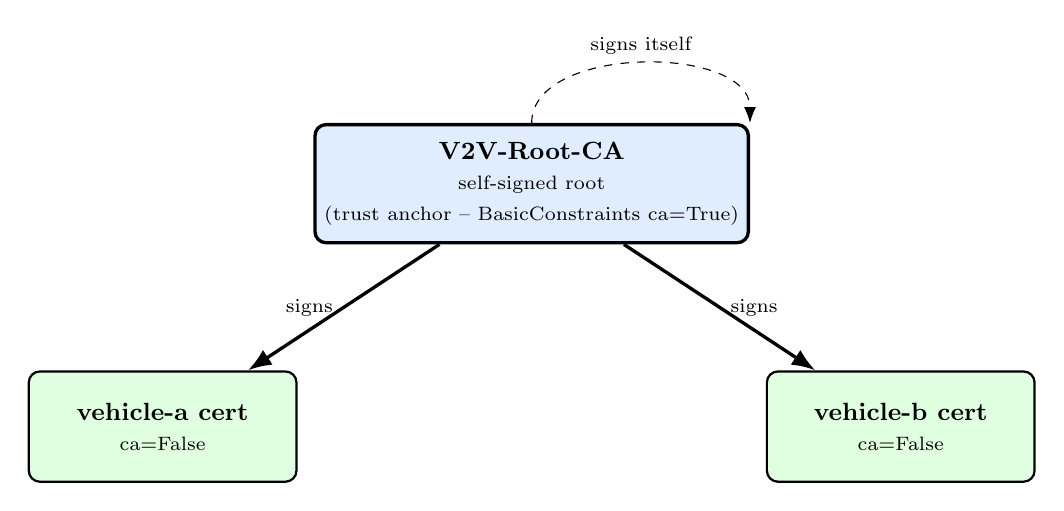
\begin{tikzpicture}[font=\small,node distance=12mm,
   ca/.style={draw,very thick,rounded corners,fill=boxblue,minimum width=4.6cm,
              minimum height=1.5cm,align=center},
   veh/.style={draw,thick,rounded corners,fill=green!12,minimum width=3.4cm,
               minimum height=1.4cm,align=center}]
  \node[ca] (ca) {\textbf{V2V-Root-CA}\\\scriptsize self-signed root\\
                   \scriptsize (trust anchor -- BasicConstraints ca=True)};
  \node[veh,below left=16mm and 2mm of ca]  (a) {\textbf{vehicle-a cert}\\\scriptsize ca=False};
  \node[veh,below right=16mm and 2mm of ca] (b) {\textbf{vehicle-b cert}\\\scriptsize ca=False};
  \draw[-{Latex[length=3mm]},very thick] (ca) -- (a)
       node[midway,left,font=\scriptsize]{signs};
  \draw[-{Latex[length=3mm]},very thick] (ca) -- (b)
       node[midway,right,font=\scriptsize]{signs};
  \draw[-{Latex[length=2mm]},dashed] (ca.north) .. controls +(0,1) and +(0,1) .. (ca.north east)
       node[midway,above,font=\scriptsize]{signs itself};
\end{tikzpicture}
\end{center}
\noindent To trust \texttt{vehicle-a}, a verifier checks just one signature:
``did V2V-Root-CA sign this?'' Trust flows down from the root.

\subsection{Diagram 2 --- Issue then Verify}
\begin{center}
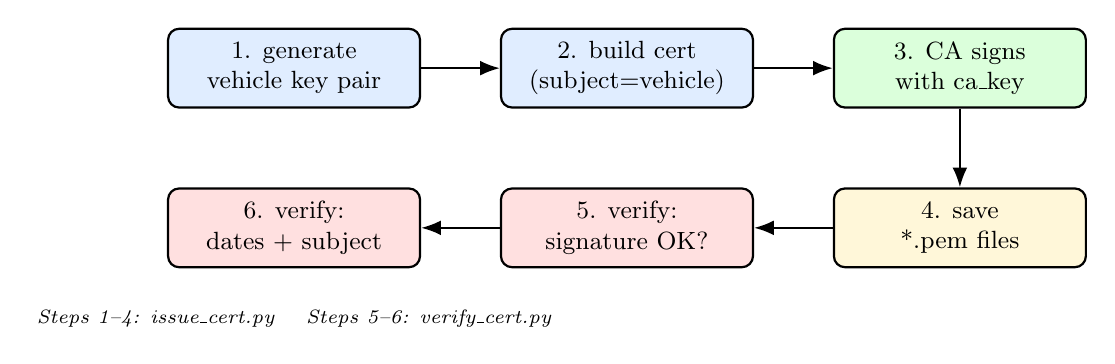
\begin{tikzpicture}[font=\small,node distance=7mm,
   box/.style={draw,thick,rounded corners,minimum width=3.2cm,minimum height=1.0cm,
               align=center}]
  \node[box,fill=boxblue]   (k)  {1. generate\\vehicle key pair};
  \node[box,fill=boxblue,right=10mm of k]   (build) {2. build cert\\(subject=vehicle)};
  \node[box,fill=green!14,right=10mm of build] (sign) {3. CA signs\\with ca\_key};
  \node[box,fill=boxyellow,below=10mm of sign] (save) {4. save\\*.pem files};
  \node[box,fill=red!12,below=10mm of build] (vsig) {5. verify:\\signature OK?};
  \node[box,fill=red!12,below=10mm of k] (vdate) {6. verify:\\dates + subject};
  \draw[-{Latex[length=2.5mm]},thick] (k) -- (build);
  \draw[-{Latex[length=2.5mm]},thick] (build) -- (sign);
  \draw[-{Latex[length=2.5mm]},thick] (sign) -- (save);
  \draw[-{Latex[length=2.5mm]},thick] (save) -- (vsig);
  \draw[-{Latex[length=2.5mm]},thick] (vsig) -- (vdate);
  \node[below=4mm of vdate,font=\scriptsize\itshape,align=left]
       {Steps 1--4: issue\_cert.py \quad Steps 5--6: verify\_cert.py};
\end{tikzpicture}
\end{center}

% =====================================================================
\section{Presentation Pack}
% =====================================================================

\subsection{Slide Outline}

\textbf{Slide 1 --- The Identity Problem.}
\begin{itemize}
  \item Two cars must trust each other before they talk.
  \item A bare public key is just a number --- it does not say \emph{whose}.
  \item We need a digital ``passport'' that cannot be faked.
  \item Solution: a Certificate Authority --- a digital passport office.
\end{itemize}

\textbf{Slide 2 --- The Certificate Authority (ca.py).}
\begin{itemize}
  \item The CA generates a P-256 key pair (\texttt{generate\_ca\_key}).
  \item It builds a \emph{self-signed} root certificate (issuer = subject).
  \item \texttt{BasicConstraints ca=True} --- it is allowed to sign others.
  \item It saves \texttt{ca\_cert.pem} (public) and \texttt{ca\_key.pem} (secret).
\end{itemize}

\textbf{Slide 3 --- Issuing a Vehicle Certificate (issue\_cert.py).}
\begin{itemize}
  \item The vehicle generates \emph{its own} key pair; the CA never sees the
        private half.
  \item The CA builds a cert with subject = vehicle, issuer = CA.
  \item \texttt{builder.sign(private\_key=ca\_key)} --- the CA's signature is the
        link in the chain of trust.
  \item Vehicle cert is \texttt{ca=False}, valid one year.
\end{itemize}

\textbf{Slide 4 --- Verifying a Certificate (verify\_cert.py).}
\begin{itemize}
  \item Three checks: signature, dates, subject.
  \item Signature check: \texttt{ca\_public\_key.verify(...)} --- the heart of it.
  \item A forged or edited certificate raises \texttt{InvalidSignature}.
  \item All three must pass $\to$ \texttt{CERTIFICATE IS VALID}.
\end{itemize}

\textbf{Slide 5 --- Why This Beats a Forged-Certificate MITM.}
\begin{itemize}
  \item Attacker has no CA private key, so cannot make a cert that verifies.
  \item Self-signed forgery $\to$ wrong signer $\to$ rejected.
  \item Edited real cert $\to$ body bytes changed $\to$ rejected.
  \item S2 (identity) + S4 (prove you own the key) together defeat MITM.
\end{itemize}

\subsection{Speaker Talking Points (about 30--60 seconds each)}

\textbf{Slide 1.} ``Before our two cars can have a secure conversation, each one
has to know it is really talking to a genuine vehicle and not an impostor. The
problem is that a public key on its own is just a long number --- it carries no
name. So we need something like a passport: a document that ties a key to an
identity and that nobody can forge. To create and check those passports we build
a Certificate Authority --- think of it as a digital passport office that
everyone agrees to trust.''

\textbf{Slide 2.} ``The file ca.py builds that authority. First it generates a
key pair on the P-256 elliptic curve --- a private key it keeps secret and a
public key it will share. Then it builds its own certificate. Because nobody
ranks above the CA, it signs that certificate with its own key --- that is what
`self-signed' means, and you can see it in the code where subject and issuer are
the same name. It marks the certificate `ca equals true', meaning this key is
allowed to sign other certificates, and saves two files: the public ca\_cert.pem,
which every vehicle gets a copy of, and the secret ca\_key.pem.''

\textbf{Slide 3.} ``Issuing a vehicle certificate is the job of issue\_cert.py.
An important detail: the vehicle generates its \emph{own} key pair --- the CA
never sees the vehicle's private key. The CA only takes the vehicle's public key,
wraps it in a certificate that names the vehicle as subject and the CA as issuer,
and then signs it with the CA's private key. That one signing line is the entire
purpose of a CA --- it is the link in the chain of trust. The vehicle certificate
is marked `ca equals false', so a vehicle can never issue certificates itself,
and it lasts one year instead of ten.''

\textbf{Slide 4.} ``verify\_cert.py is the border guard. It runs three checks.
The date check makes sure the certificate has not expired. The subject check
reads out who it belongs to. But the real test is the signature check: it takes
the CA's public key and asks `did the matching CA private key sign this exact
certificate body?'. If yes, it passes silently. If the certificate was forged or
even slightly edited, the library raises an InvalidSignature error and we reject
it. Only if all three checks pass do we print CERTIFICATE IS VALID.''

\textbf{Slide 5.} ``Here is why this defeats a man-in-the-middle who tries a fake
certificate. To make a certificate that passes our signature check, the attacker
would need the CA's private key --- and that key never leaves the CA. If they
self-sign a fake, it was signed by the wrong key and is rejected. If they edit a
real certificate, the body bytes change and the old signature no longer matches,
so it is rejected too. Section S2 proves \emph{identity}; Section S4 then makes
the vehicle prove it actually \emph{owns} the private key. Together they shut the
door on man-in-the-middle.''

\subsection{Live-Demo Script}
\begin{enumerate}
  \item \textbf{Build the CA.} Run \texttt{python ca\textbackslash ca.py}. Point
        at the line where Subject equals Issuer and say ``this is self-signed.''
  \item \textbf{Issue two certificates.} Run the two
        \texttt{issue\_cert.py} commands. Point at ``Certificate signed by CA''
        and at the SHA-256 fingerprint.
  \item \textbf{Verify a good certificate.} Run \texttt{verify\_cert.py} on
        \texttt{vehicle-a}. Point at the three \texttt{[OK]} lines and
        \texttt{CERTIFICATE IS VALID}.
  \item \textbf{Break it live.} Open \texttt{vehicle-a\_cert.pem}, change one
        Base64 character, save, re-run verify. Point at
        \texttt{[FAIL] Signature invalid} --- ``this is what happens to every
        forgery.'' Then re-issue the certificate to restore it.
\end{enumerate}

\subsection{Examiner Q\&A}
\begin{enumerate}
  \item \textbf{Q: What is a Certificate Authority?}\\
        A: A trusted party that issues and signs certificates --- a digital
        passport office. In this project it is created by \texttt{ca.py} and is
        named \texttt{V2V-Root-CA}.
  \item \textbf{Q: What does ``self-signed'' mean and why is the root self-signed?}\\
        A: The certificate's issuer and subject are the same, and it is signed
        with its own private key. The root is self-signed because nothing ranks
        above it; trust in the root must be established out-of-band by
        distributing \texttt{ca\_cert.pem}.
  \item \textbf{Q: Does the CA ever see a vehicle's private key?}\\
        A: No. The vehicle generates its own key pair in
        \texttt{generate\_vehicle\_key}; only the \emph{public} key is sent to
        the CA to be placed in the certificate and signed.
  \item \textbf{Q: How does \texttt{verify\_cert.py} detect a forged certificate?}\\
        A: \texttt{check\_signature} calls \texttt{ca\_public\_key.verify} over
        \texttt{tbs\_certificate\_bytes}. A forgery was not signed by the CA's
        private key, so verification raises \texttt{InvalidSignature}.
  \item \textbf{Q: What are \texttt{tbs\_certificate\_bytes}?}\\
        A: ``To Be Signed'' --- the exact certificate body bytes that the
        signature covers (everything except the signature itself). Verifying
        re-hashes these bytes and checks them against the signature.
  \item \textbf{Q: What do BasicConstraints and KeyUsage do?}\\
        A: BasicConstraints \texttt{ca=True/False} says whether the certificate
        may sign other certificates. KeyUsage limits the key's job ---
        \texttt{key\_cert\_sign} for the CA, \texttt{digital\_signature} for a
        vehicle. Marked critical, so a verifier must honour them.
  \item \textbf{Q: What is PEM and how does it differ from DER?}\\
        A: DER is the raw binary encoding; PEM is that binary Base64-encoded as
        text and wrapped in BEGIN/END lines so it survives copy-paste and email.
  \item \textbf{Q: Name one realistic weakness of this CA design.}\\
        A: \texttt{ca\_key.pem} is stored unencrypted (\texttt{NoEncryption()}),
        so anyone who reads that file controls the whole PKI. A real CA encrypts
        the key or keeps it in a Hardware Security Module. Also there is no
        revocation (no CRL/OCSP) --- a compromised vehicle certificate cannot be
        cancelled before it expires.
\end{enumerate}

% =====================================================================
\section{Glossary}
% =====================================================================
\begin{description}[style=nextline,leftmargin=0pt]
  \item[PKI] Public Key Infrastructure: the system of CAs, certificates and
        rules that lets strangers trust public keys.
  \item[CA] Certificate Authority: the trusted issuer and signer of certificates.
  \item[Certificate (X.509)] A standard digital document binding an identity to
        a public key, signed by an issuer.
  \item[Symmetric cryptography] One shared secret key for both locking and unlocking.
  \item[Asymmetric / public-key cryptography] A key pair: a private key kept
        secret and a public key shared freely.
  \item[Private key] The secret half of a key pair; used to sign.
  \item[Public key] The shareable half of a key pair; used to verify.
  \item[ECC] Elliptic-Curve Cryptography: public-key crypto based on curve maths.
  \item[P-256 / SECP256R1] The specific NIST elliptic curve used in this project.
  \item[SHA-256] A hash function producing a 256-bit fixed-size fingerprint.
  \item[Hash function] A one-way function turning any data into a short fingerprint.
  \item[Digital signature] A value made with a private key and checkable with the
        public key, proving authorship and integrity.
  \item[ECDSA] Elliptic Curve Digital Signature Algorithm.
  \item[Self-signed] A certificate whose issuer and subject are the same; signed
        with its own key.
  \item[Chain of trust] The line of signatures from a certificate back to a
        trusted root.
  \item[Trust anchor / root] The already-trusted certificate at the top of a chain.
  \item[Subject] Who a certificate is about.
  \item[Issuer] Who signed a certificate.
  \item[Serial number] A unique number identifying a certificate.
  \item[Fingerprint] A SHA-256 hash of a whole finished certificate, for human comparison.
  \item[BasicConstraints] Extension stating whether a certificate is a CA.
  \item[KeyUsage] Extension stating what a key is allowed to do.
  \item[Critical extension] An extension a verifier must understand or reject the cert.
  \item[Validity period] The not-before / not-after dates of a certificate.
  \item[DER] The compact binary encoding of a certificate or key.
  \item[Base64] A text encoding of binary data using 64 printable characters.
  \item[PEM] A text format: Base64 wrapped in BEGIN/END header lines.
  \item[tbs\_certificate\_bytes] The ``to-be-signed'' body bytes a signature covers.
  \item[HSM] Hardware Security Module: tamper-proof hardware for storing keys.
  \item[CRL / OCSP] Mechanisms for revoking (cancelling) a certificate early ---
        not implemented in this project.
\end{description}

% =====================================================================
\section{References and Further Study}
% =====================================================================
\begin{itemize}
  \item \textbf{Public Key Infrastructure (Wikipedia)} ---
        \url{https://en.wikipedia.org/wiki/Public_key_infrastructure}\\
        Read for: the big picture of CAs, certificates and trust.
  \item \textbf{X.509 (Wikipedia)} ---
        \url{https://en.wikipedia.org/wiki/X.509}\\
        Read for: the certificate format, fields and extensions.
  \item \textbf{RFC 5280 --- Internet X.509 Certificate Profile} ---
        \url{https://datatracker.ietf.org/doc/html/rfc5280}\\
        Read for: the authoritative definition of X.509 certificates and
        BasicConstraints / KeyUsage.
  \item \textbf{Public-key cryptography (Wikipedia)} ---
        \url{https://en.wikipedia.org/wiki/Public-key_cryptography}\\
        Read for: how key pairs work and why public keys are safe to share.
  \item \textbf{Elliptic-curve cryptography (Wikipedia)} ---
        \url{https://en.wikipedia.org/wiki/Elliptic-curve_cryptography}\\
        Read for: a gentle introduction to ECC.
  \item \textbf{ECDSA (Wikipedia)} ---
        \url{https://en.wikipedia.org/wiki/Elliptic_Curve_Digital_Signature_Algorithm}\\
        Read for: how elliptic-curve signatures sign and verify.
  \item \textbf{NIST FIPS 186-5 --- Digital Signature Standard} ---
        \url{https://csrc.nist.gov/pubs/fips/186-5/final}\\
        Read for: the official standard behind ECDSA and the P-256 curve.
  \item \textbf{SHA-2 / SHA-256 (Wikipedia)} ---
        \url{https://en.wikipedia.org/wiki/SHA-2}\\
        Read for: how the hash function used in signing works.
  \item \textbf{PEM / DER explained (Python cryptography docs)} ---
        \url{https://cryptography.io/en/latest/x509/}\\
        Read for: how this project's exact library handles certificates and PEM.
  \item \textbf{Python cryptography --- X.509 reference} ---
        \url{https://cryptography.io/en/latest/x509/reference/}\\
        Read for: \texttt{CertificateBuilder}, \texttt{load\_pem\_x509\_certificate},
        and every API used in S2.
  \item \textbf{Computerphile --- ``Public Key Cryptography'' (video)} ---
        \url{https://www.youtube.com/watch?v=GSIDS_lvRv4}\\
        Read/watch for: an intuitive, visual explanation of key pairs.
\end{itemize}

\vfill
\begin{center}\footnotesize\itshape
End of Section S2. Next: S3 --- the Cryptographic Core (AES-GCM, ECDH, HKDF, ECDSA).
\end{center}

\end{document}
